\section{Tacit and Latent Needs}\label{sec:codesign:part2}
%Participatory Design of Password Feedback
% continue rapid approach from first study 
As second step of the co-creation project, we aimed to learn from specific user-generated designs and solutions. Therefore, we took to the participatory design methodology. In its essence, it is a technique that constitutes a ``shift in attitude from designing \textbf{for} users to one of designing \textbf{with} users'' \cite{Sanders2002ParticipatoryDesign}. Therefore, having identified a research question, users from the targeted segment are involved from the beginning in design explorations and create their own solutions (``Make'' in Figure \ref{fig:co-design:exploration-overview}). Moreover, a tight feedback loop makes sure that all designs are created under a \textit{shared ownership}. In our case, we were eager to find out what a novel password support system could look like. In particular, unusual and exciting ideas beyond simple password meters were the center of attention. The overarching goal was to identify \textbf{what users require} from password feedback systems, which would help us design them in more persuasive ways.

%\begin{figure}[htbp]
%	\centering
%	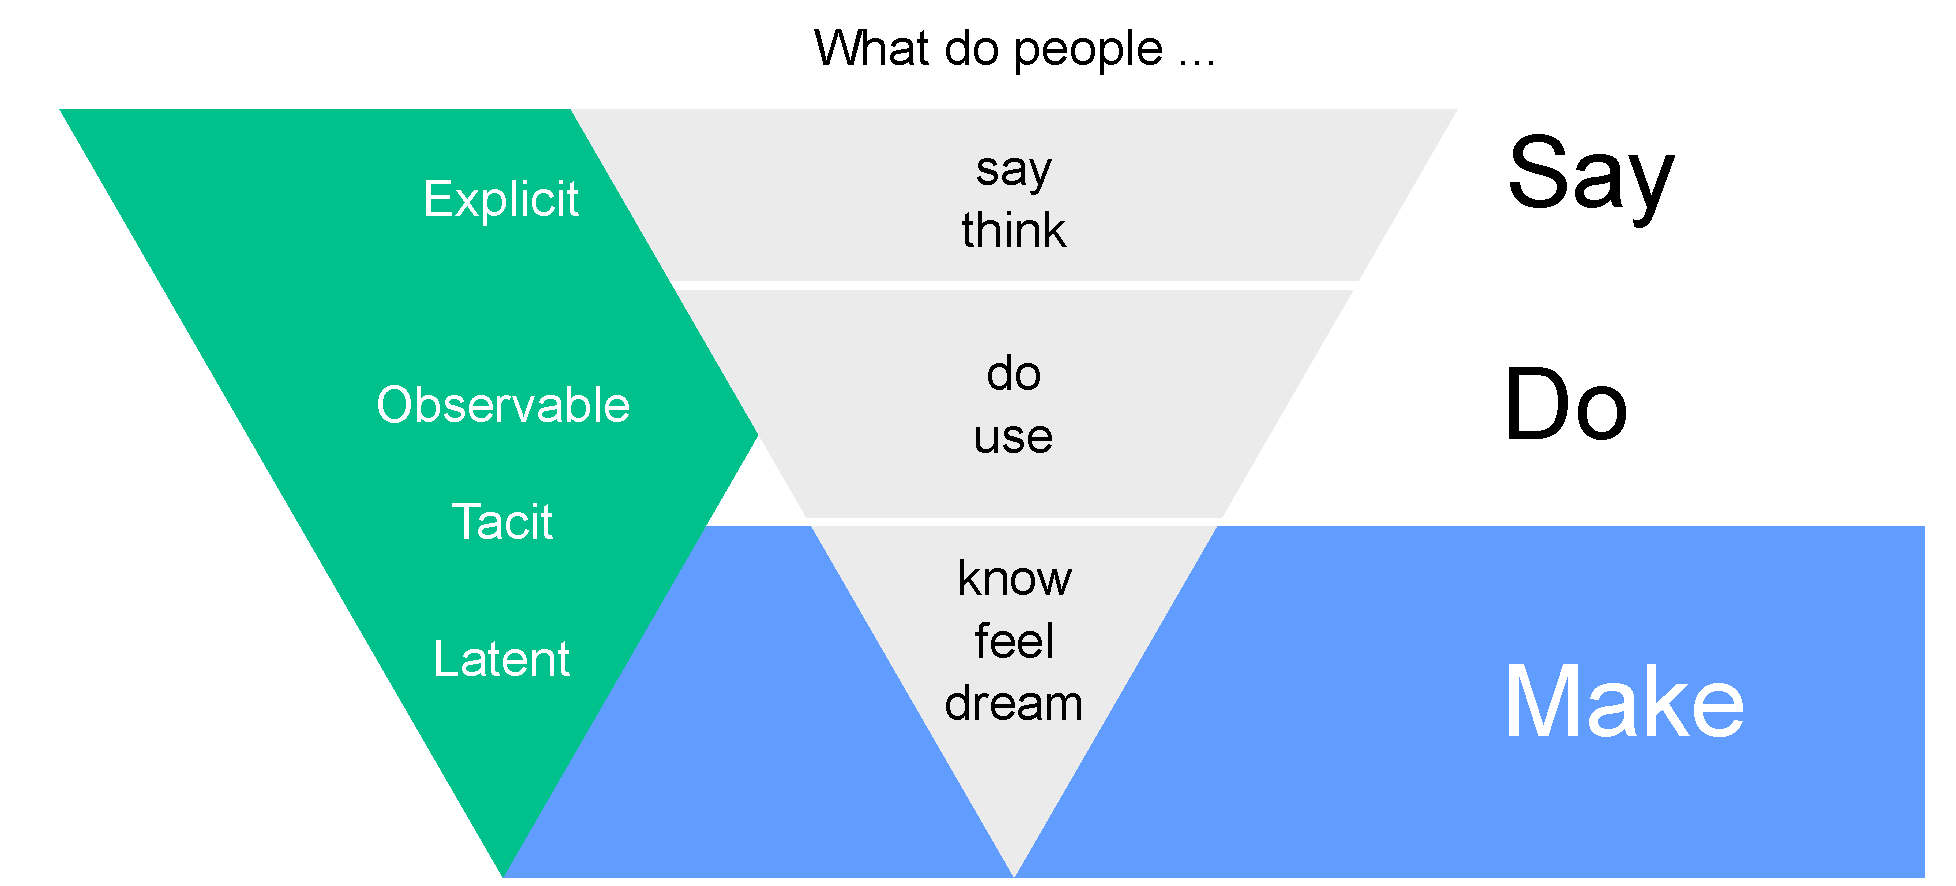
\includegraphics[width=0.8\linewidth]{figures/co-design/participatory-needs}
%	\caption{\label{fig:co-design:participatory-needs} This project focused on understanding user needs by learning from what they \textbf{make}.}
%\end{figure}


%GOAL: design session to actually teach us more about the requirements, not necessarily about the solutions. The prototypical and conjoint solutions tell us about the expectations and needs of users regarding password feedback. 

%todo maybe pick up the insights from the previous survey

%- Involve users in the design of a novel feedback solution
%- participatory design session
%- different groups

\subsection{Method}
We used the participatory design approach to learn new requirements for persuasive feedback. The methodology included a co-design session with various exercises, an exploration and refinement of the initial ideas, a feedback loop on the progress of the concepts, and the creation of a final interactive digital prototype.

\subsubsection{Procedure of the Co-Design Session}
%Brainstorming Session, 60 minutes, different exercises, keep tempo high.
% 1
The 60-minute co-design session started with a briefing about the goals and informed consent to record the session on video. Afterwards, we sensitized participants for the topic with two \textit{ball-bearing exercises}. For this, participants were divided into two groups and those faced each other in a circle. Each person interviewed another on a specific question of password behavior for one minute. The outer circle moved to the next interviewer until they had talked to all people from the inner circle. In the first round, interviewers were given questions on personal password selection and coping strategies. The second round focused on recommendations to different user groups. The interviewers then summarized their insights and shared them with the group. The exercise was helpful to learn other people's password strategies and broaden the participants' horizon. They said it was interesting to reflect about obstacles in acting more securely. In summary, participants showed typical selection strategies based on word-digit-symbol patterns and would recommend personal, memorable events as starting points for password selection.

What followed were straightforward brainstorming exercises in two groups. The question they tried to answer was ``How would a registration form of an email provider need to be designed to help you create a secure password?'' The facilitator encouraged participants to think out of the box and contribute unusual ideas. After five minutes, half of each group moved to the other group. In total, participants produced 17 distinct ideas and presented them on a whiteboard. Everyone received two votes for their favorite ideas. Participants then formed groups of two or three to create paper prototypes for the three ideas that had the most votes. The facilitator made sure to explain the process and the expected fidelity of the outcome. Once the prototypes were ready, the groups presented them to the entire crowd.

\paragraph{Participants}
We recruited seven participants through postings in public groups on social networks. Six of them were female. Three were studying philology, while one each were studying pedagogy, media informatics and business studies. The only male participant was an employed product designer. The average age was 23, ranging from 19 to 29. As an incentive, we offered a 10€ shopping voucher that was handed out after the brainstorming session. We had tried to recruit a more diverse sample, but we did not receive additional responses meeting these requirements. 

\subsubsection{10 plus 10 Method and Iterative Improvement}
Based on the participants' paper prototypes, we designed ten variations of each idea, i.e. 30 concept candidates. This procedure was inspired by the \textit{10 plus 10 method} to explore the design space\footurl{http://sketchbook.cpsc.ucalgary.ca/wp-content/uploads/Chapter-1.4-10Plus10Method.ppt}{24.04.2018}. 
Afterwards, we discussed the feasibility of each solution and identified six candidates that were presented to the study participants. Their feedback informed the decision on the final prototype. After it was implemented with standard web-technologies, participants provided a final round of qualitative feedback and a reflection on the process. Participation thus occurred in each step of the design process. 

\subsection{Concepts and Prototype}
The paper prototypes of the brainstorming session showed three central components: \textbf{rewards}, \textbf{analogies and compliance}, and \textbf{playfulness}. After the 10 plus 10 method, we had six candidates that made it to the final feedback round, two of each category. Please note that we tried to stay as close to the participants' original ideas as possible and maintained concepts that were unrealistic. 
\paragraph{Rewards} The ``beautify'' concept removed all color from the website and faded it back in as the entered password increases in strength. The ``friends'' concept would provide a password meter that uses pictures of the user's friends instead of color to reward stronger passwords and add a personal touch. 
\paragraph{Analogies and Compliance}
Concepts in this category tried to nudge users by making strength more graspable and salient. The ``songs'' concept shows the number of songs that one can listen to until an attacker would have cracked the password. The ``fruits'' concept (see Figure \ref{fig:co-design:fruitsalad}) draws from a healthy-eating analogy and represents each character type with a fruit. While the user types, fruits are ``plucked'' from a character patch and moved to the password field. If a password only contains lowercase letters, the lack of complexity is immediately visible because only one type of fruit would have been plucked. 
\paragraph{Playfulness} The ``slotmachine'' idea lets the user first enter a password. Then they pull the lever of a virtual slotmachine. When it stops, it displays four random characters that would make the password stronger. The user can then claim the win by adding the random characters to their password. Finally, the ``bubbles'' concept lets the user burst bubbles floating on the screen (see Figure \ref{fig:co-design:bubbles-concept}). Inside each bubble, there is either a letter, digit, or symbol. The user can click on them directly to transfer the corresponding character to the password field, or burst bubbles by typing on the keyboard. The longer the password, the fewer bubbles remain. Also, less common character classes are shown in bigger bubbles to persuade users to burst those and hereby increase complexity. 

\begin{figure}
	\centering
	\begin{subfigure}[!t]{0.49\textwidth}
		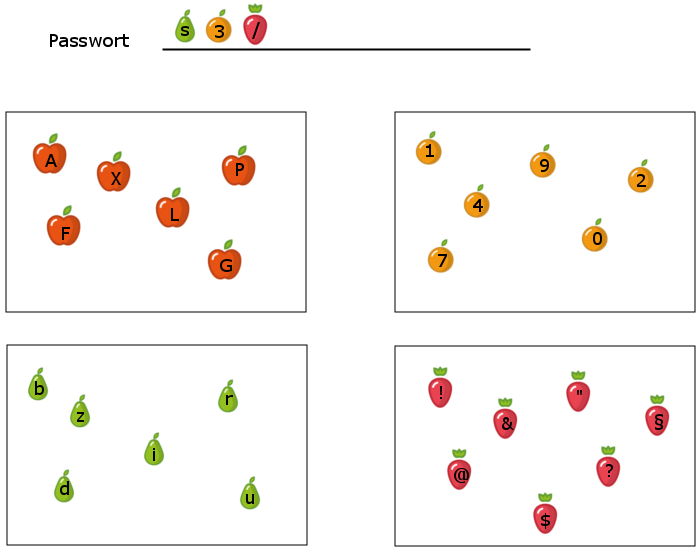
\includegraphics[width=\textwidth]{figures/co-design/fruitsalad-1}
		\caption{\label{fig:co-design:fruitsalad} Fruitsalad: Each character class is represented by a fruit and the user sees a lack of diversity, e.g. if their password only contains lowercase letters.}
	\end{subfigure}
	\begin{subfigure}[!t]{0.49\textwidth}
		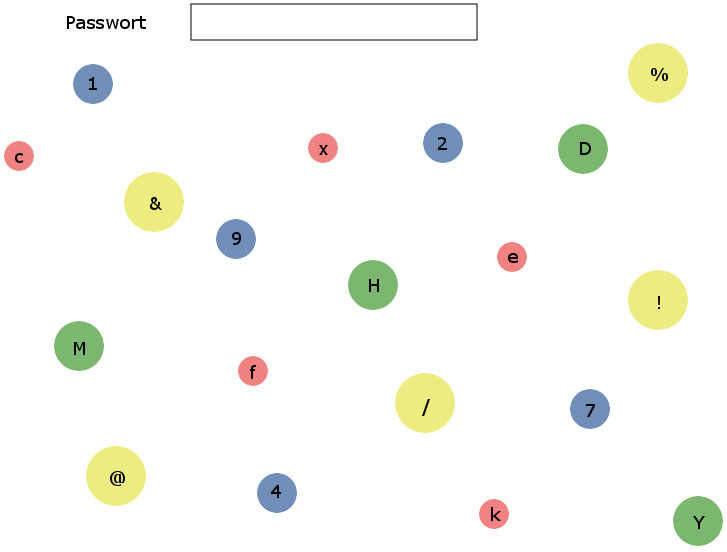
\includegraphics[width=\textwidth]{figures/co-design/bubbles-1}
		\caption{\label{fig:co-design:bubbles-concept}Bubbles: Floating bubbles on the screen that the user pops as they type the password. Symbols are placed in bigger bubbles to be more salient.}
	\end{subfigure}
	\caption{\label{fig:co-design:concepts}Two out of the six concepts that made it to the final feedback iteration.} 
\end{figure}


%- Designs:
%- rewards: beautify page / positive reinforcement from friends (weird suggestions but okay)
%- analogies and requirements feedback: time to crack --> goal: better risk assessment for non-experts. / represent strength contribution of different elements in some way (fruit salad) / vault 
%- playfulness: bubbles / vault / slotmachine to make random character replacements more exciting / 
\subsubsection{``Bubbles'' Prototype}
Participants provided feedback on the six concepts and generally considered the ``bubbles'' concept the best solution to motivate themselves to add more symbols or digits and also make the password longer to watch more bubbles burst. Therefore, we implemented it as an HTML5-based prototype. To add a more game-like feel, we put a score on each character class, and show the currently achieved total score in the GUI. The bubbles move slowly enough to trace them and their bursts. 

Five of the participants provided a final round of feedback. On the positive side, they felt it intriguing to burst the bubbles. They understood the purpose of the bubbles and the different sizes and colors right away or after typing the first character. Two participants noted that it fosters creativity. All said that a system like this would catch their eye and might impact their selection behavior. They also mentioned a number of improvements. For instance, two participants fount the page chaotic and wanted it simplified. The scoring was not transparent either, and three said the bursting animation should be more obtrusive. 

\begin{figure}
	\centering
	\begin{subfigure}[!t]{0.45\textwidth}
		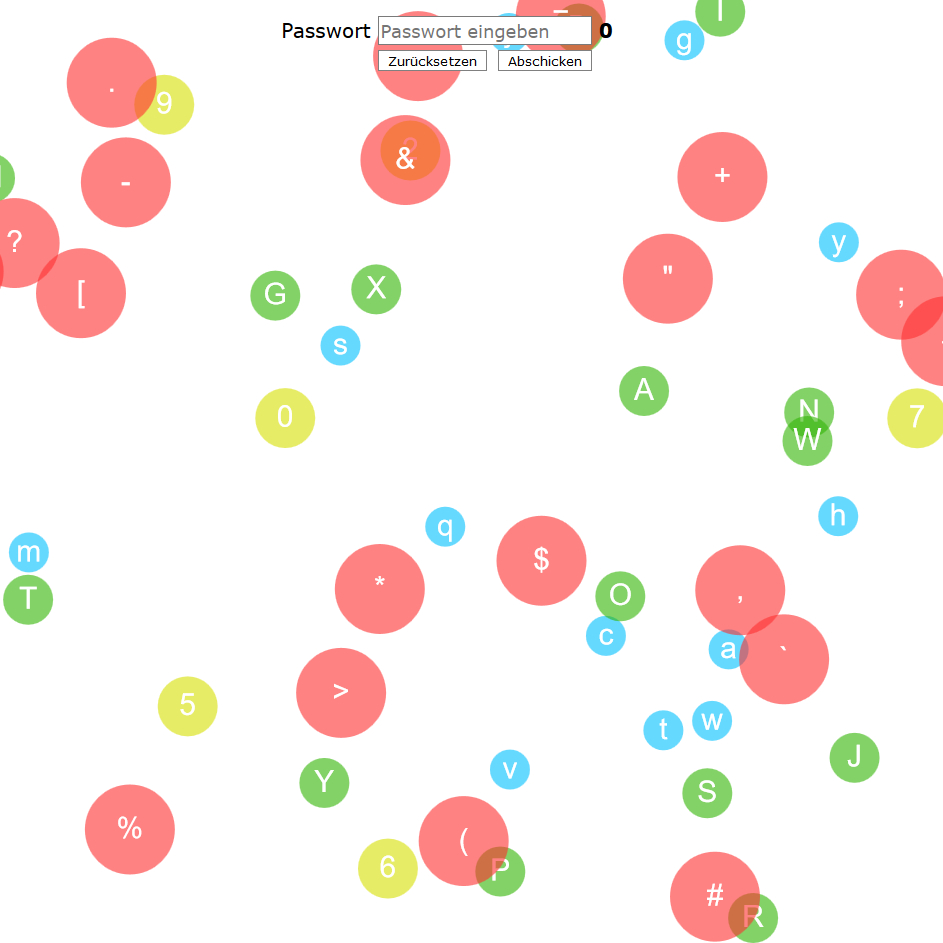
\includegraphics[width=\textwidth]{figures/co-design/bubbles-proto-1}
		\caption{\label{fig:co-design:bubbles-proto-1}}
	\end{subfigure}
	\begin{subfigure}[!t]{0.45\textwidth}
		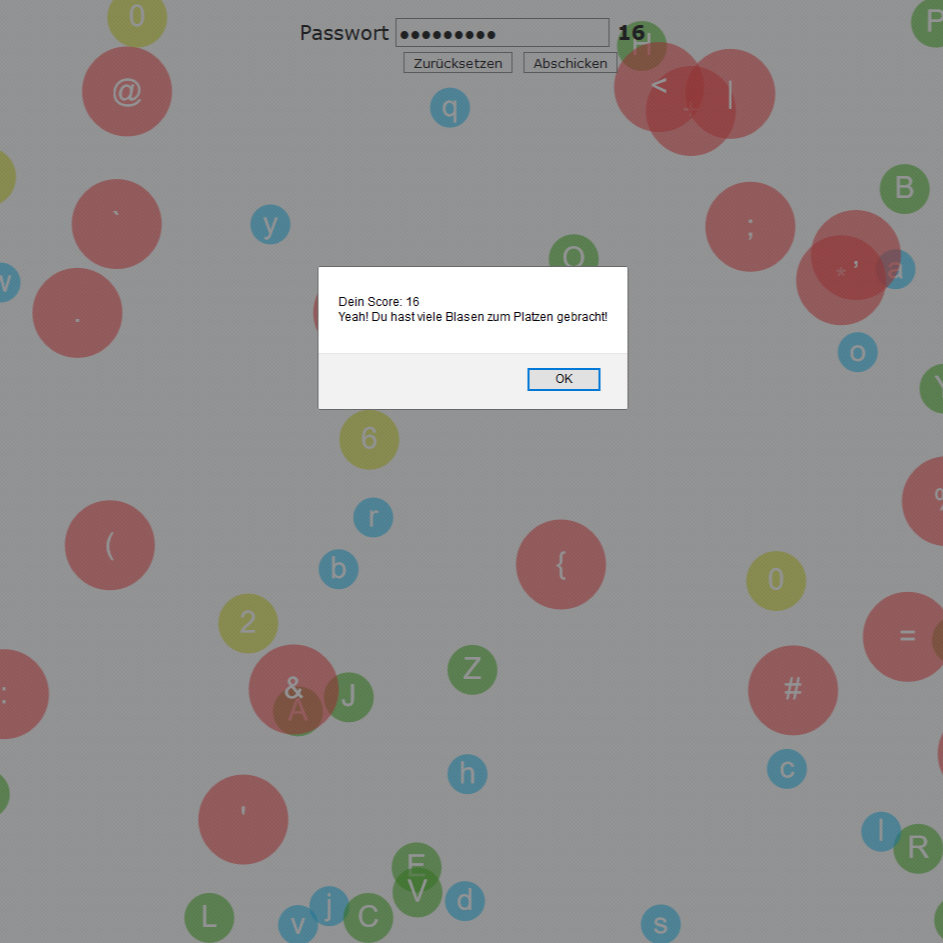
\includegraphics[width=\textwidth]{figures/co-design/bubbles-proto-2}
		\caption{\label{fig:co-design:bubbles-proto-2}}
	\end{subfigure}
	\caption{\label{fig:co-design:bubbles-proto} We made the ``bubbles'' concept into an interactive prototype and gathered a final round of feedback on the outcome and the process.} 
\end{figure}

\subsection{Process Reflection}
Participants were also asked to provide feedback about their experiences along the way. Generally, they were positive and felt involved generating a new design. They reported that the final prototype reflected the entire process well and that elements from the idea generation stages were visible. In particular, they liked to think about finding solutions to a problem that they had not thought about in depth. Three of them said that they would have still liked more involvement so that they can shape the outcome even more. One participant, on the other hand, said that s/he disliked that most ideas were far-fetched and too unrealistic. S/he would have liked a more product-centric development process.

\subsection{Lessons about Persuasive Password Interventions}
Discussions among participants and their continuous feedback throughout the design process helped us understand various user needs. We heard that the group had not given the topic much thought before joining the brainstorming session. Many of their ideas went beyond typical password meters, which we highly encouraged. In particular, the concepts show a tendency to \textbf{visual elements} (beautify, pictures, bubbles, fruits) to catch the user's attention. This corresponds to the \textit{show} theme of the requirement-elicitation. The \textit{help} theme was visible especially in the compliance-centered concepts: The ``fruit-salad'' supports people in recognizing a potential lack of character diversity. While the ``songs'' analogy is a kind of \textit{explanation} of password strength because it gives background information, the ideas did not contain many attempts to explain additional aspects. Perhaps, participants equated strength with complexity -- a mental model that we found in Chapter \ref{chap:pasdjo} -- and their ideas confirmed this thinking model. Finally, the ``bubbles'' concept aimed to boost creativity and thus showed elements of the \textit{help} and \textit{empower} themes. 

%- interesting aspects:
%- a lot of the concepts are visualizable with little text. (emphasize: ``show'' and ``help'')
%- missing: background information. (thus ``explain'' was not visible anymore)
%- empower: not really visible
%kicked out content / structure
% 2
%Ball-bearning exercise
%- add picture of concept: two circles, people on the inner circle interview those on the outer circle who move along after 2 minutes. inner circle gets 1-2 minutes to summarize their findings. 
%- purpose: 
%- first round: own behavior and practices
%- what do (other) people know about password strength and feedback, 
%- what do they do to create passwords
%- share experiences
%- take away: mangling words
%- second round: if they were asked by other people (grandmother, relatives, friends/peers)
%- take away: use context or a good memory as a starting point for your password, e.g. the location and year of a treasured vacation
%- explore potential problems of users, share stories
%- facilitator comments on findings.

%\% 3 
%Idea generation
%- task: ``how would a registration form on a webpage have to look, to help you create a secure password?'' context: email provider
%- quantity!
%- 2x5 minutes in different groups
%- put central topics on whiteboard (17 ideas from both rounds)
%
%\% 4 converge
%- everyone votes for their favorite (2 votes) --> here 3 ideas with 4 votes each were the winners
%- groups of 2 or 3 to build a paper prototype (after a brief explanation what that is)
%
%\% 5 present
%- brief presentation of prototype
%- voting for favorites to inform what we should explore further. 